% !TEX root = ../DDL_report.tex
\section{Ход работы}

По итогам предыдущей работы была разработана SQL-схема БД для музыкальной библиотеки (\vref{pic:scheme}).

\begin{figure}[ht]
	\centering
	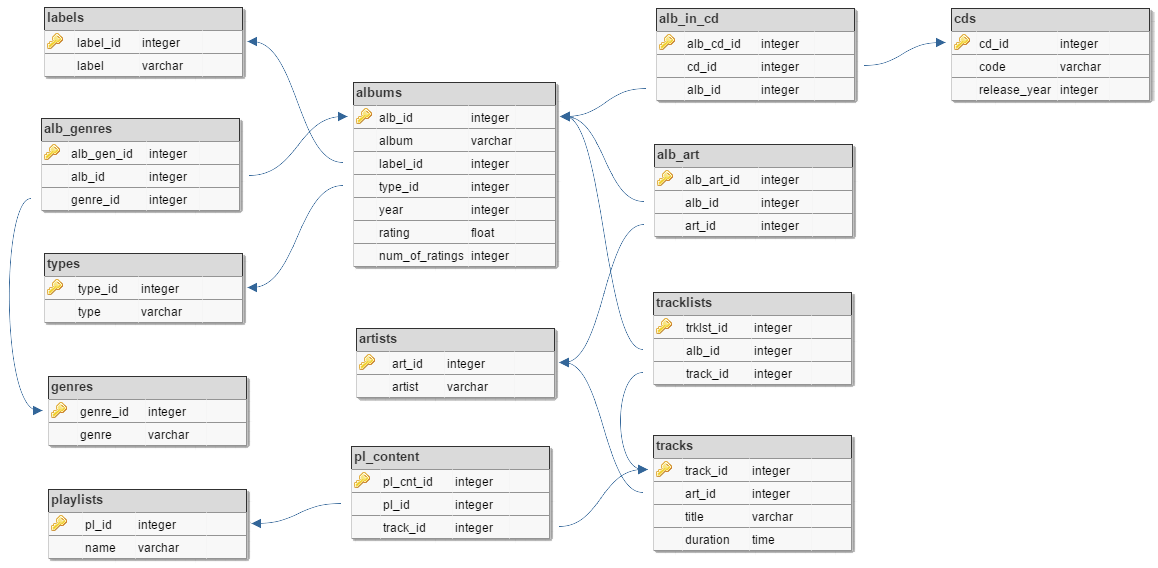
\includegraphics[width=\textwidth]{scheme}
	\caption{SQL-схема БД}
	\label{pic:scheme}
\end{figure}

На основе данной схемы был написан скрипт, создающий соответствующую структуру БД (листинг \vref{lst:create}).

\lstinputlisting[language=SQL, morekeywords={REFERENCES}, label=lst:create, caption=Скрипт для создания БД]{code/create.sql}

Далее был написан скрипт, заполняющий все таблицы БД осмысленными данными (листинг \vref{lst:fill}).

\lstinputlisting[language=SQL, morekeywords={REFERENCES}, label=lst:fill, caption=Заполнение БД]{code/fill.sql}

\section{Индивидуальное задание}

\begin{enumerate}
	\item Реализовать учет продаж дисков по странам, городам с учетом даты.
	\item Реализовать учет наград за трек, альбом.
\end{enumerate}

Для выполнения первого пункта задания были созданы 4 таблицы: city\_list (список городов), country\_list (список стран), cities\_in\_country (принадлежность городов странам) и selling (учет продаж). Таблица selling имеет внешние ключи на диск и город, а также поля количества проданных дисков и даты продажи. Учет продаж по странам можно будет реализовать в дальнейшем с помощью SQL-запроса.

Для выполнения второго пункта задания были созданы 3 таблицы: awards (для хранения названий наград), alb\_awards (учет наград для альбома) и track\_awards (учет наград для треков). Создание двух таблиц учета наград мотивируется независимостью наград, выданных одному треку из альбома, и наград, которых заслужил весь альбом целиком. \\

Таким образом, была получена модифицированная SQL-схема, представленная на \vref{pic:scheme_m}, а также написан скрипт модификации БД (листинг \vref{lst:mod}).

\begin{figure}[H]
	\centering
	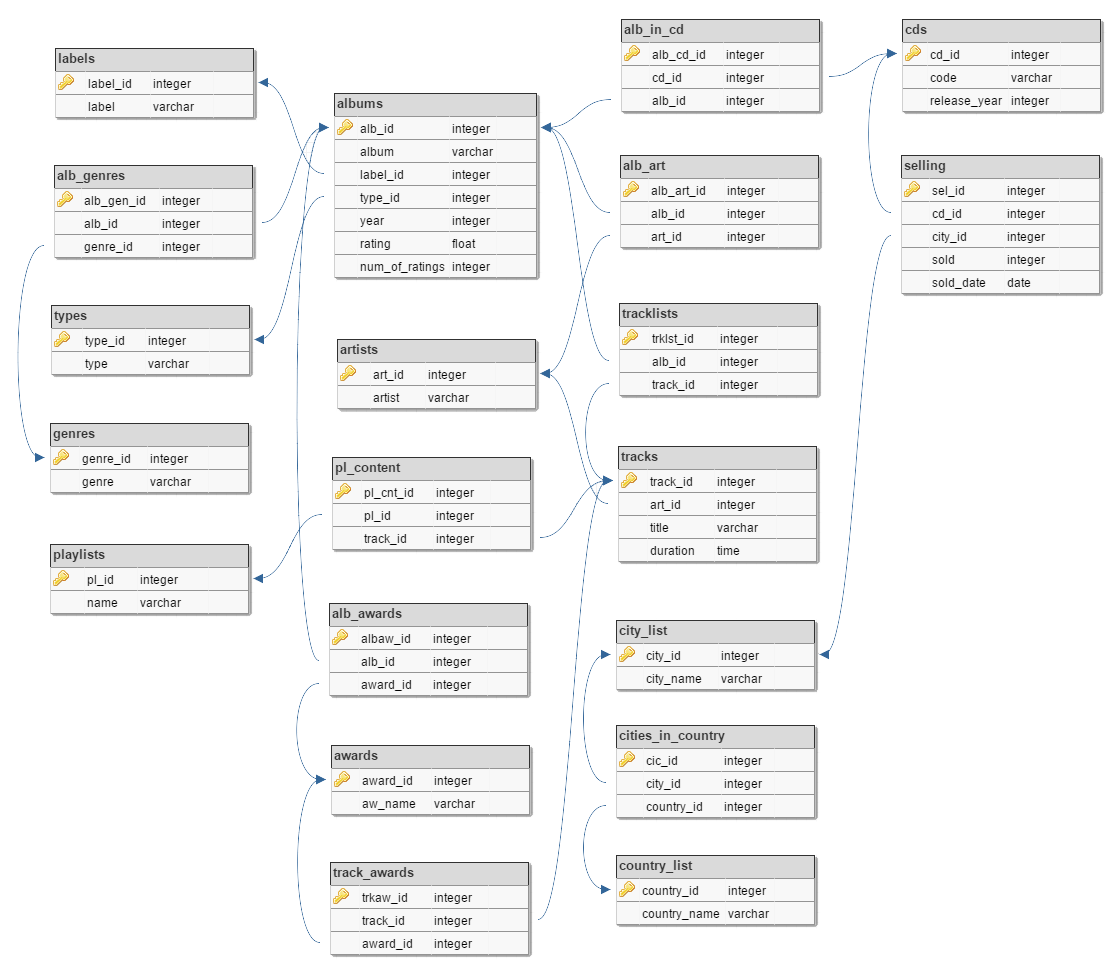
\includegraphics[width=\textwidth]{scheme_m}
	\caption{Модифицированная SQL-схема БД}
	\label{pic:scheme_m}
\end{figure}

\lstinputlisting[language=SQL, morekeywords={REFERENCES}, label=lst:mod, caption=Скрипт модификации БД]{code/mod.sql}

Дополнительно приведена ER-диаграмма, созданная с помощью инструмента Database Designer (\vref{pic:ibediagram}).

\begin{figure}[ht]
	\centering
	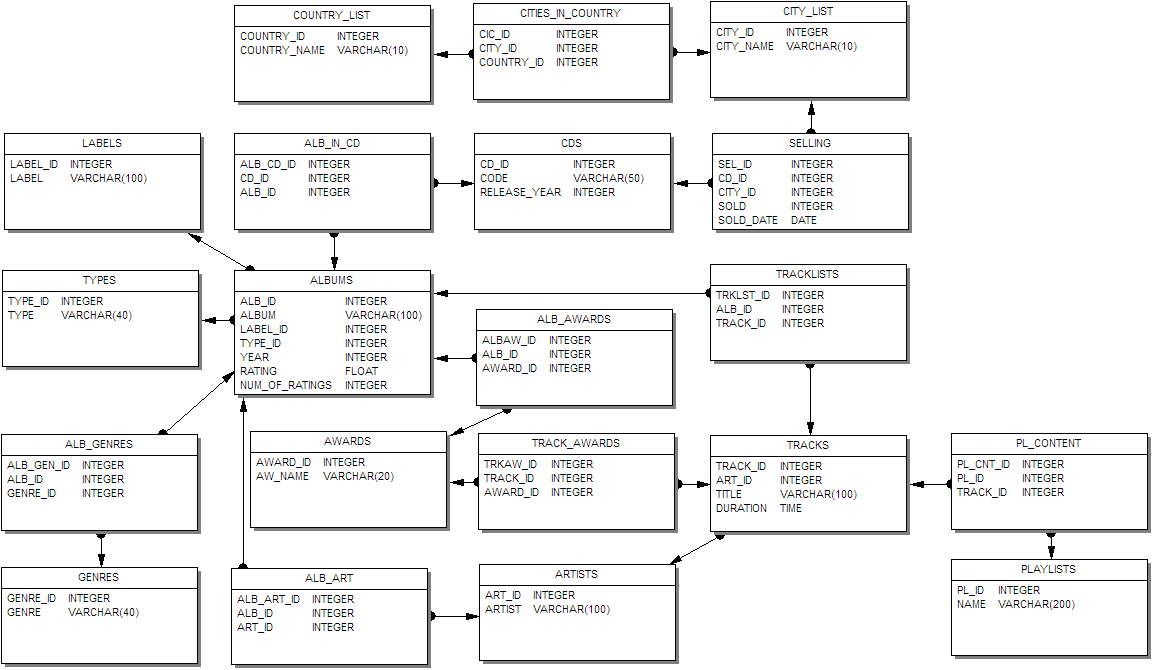
\includegraphics[width=\textwidth]{ibediagram}
	\caption{ER-диаграмма}
	\label{pic:ibediagram}
\end{figure}

Для заполнения БД случайными значениями был использован инструмент Test Data Generator. С его помощью было создано 100000 записей в таблицы albums, tracks, tracklists. Внешний вид данного инструмента представлен на \vref{pic:inc}. Для генерации выбирается таблица, количество записей, выбор полей, для которых будет происходить генерирование значений, и тип генерации полей (\vref{pic:gen}).

\begin{figure}[ht]
	\centering
	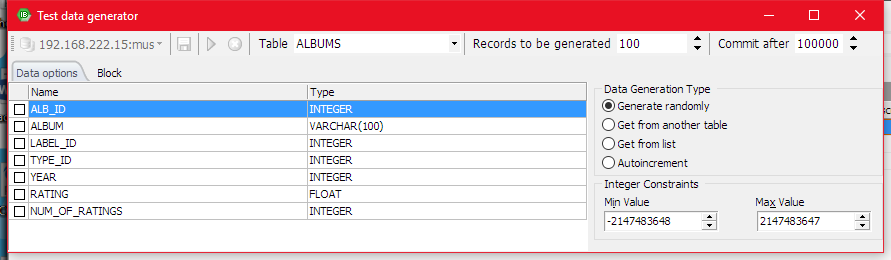
\includegraphics[width=\textwidth]{inc}
	\caption{Внешний вид Test Data Generator}
	\label{pic:inc}
\end{figure}

\begin{figure}[H]
	\begin{subfigure}{.5\linewidth}
		\centering
		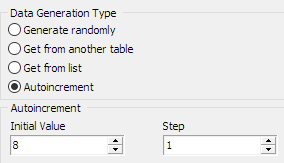
\includegraphics[width=1\textwidth]{inc2}
		\caption{Автоинкремент для первичного ключа}
		\label{pic:inc2}
	\end{subfigure}
	\begin{subfigure}{.5\linewidth}
		\centering
		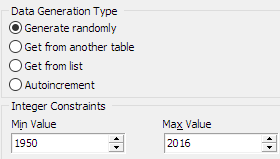
\includegraphics[width=1\textwidth]{range}
		\caption{Генерация по диапазону}
		\label{pic:range}
	\end{subfigure}
	\begin{subfigure}{.5\linewidth}
		\centering
		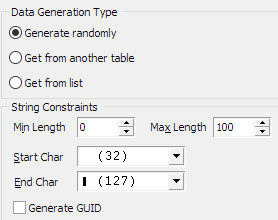
\includegraphics[width=1\textwidth]{varchar}
		\caption{Генерация VARCHAR}
		\label{pic:varchar}
	\end{subfigure}
	\begin{subfigure}{.5\linewidth}
		\centering
		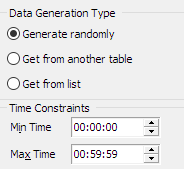
\includegraphics[width=1\textwidth]{time}
		\caption{Генерация времени}
		\label{pic:time}
	\end{subfigure}
	\begin{subfigure}{.5\linewidth}
		\centering
		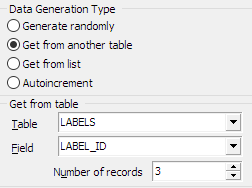
\includegraphics[width=1\textwidth]{fromtable}
		\caption{Генерация с помощью данных из другой таблицы}
		\label{pic:fromtable}
	\end{subfigure}
	\begin{subfigure}{.5\linewidth}
		\centering
		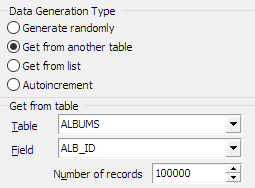
\includegraphics[width=1\textwidth]{numrec}
		\caption{Указание длины выборки значений для генерации}
		\label{pic:numrec}
	\end{subfigure}
\caption{Генерация значений в Test Data Generator}
\label{pic:gen}
\end{figure}

Пример результатов выполнения генерации представлены на \vrefrange{pic:gensuc}{pic:restrk}.

\begin{figure}[ht]
	\centering
	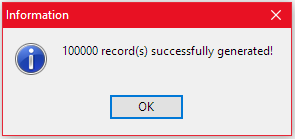
\includegraphics[width=0.4\textwidth]{gensuc}
	\caption{Завершение генерации}
	\label{pic:gensuc}
\end{figure}

\begin{figure}[ht]
	\centering
	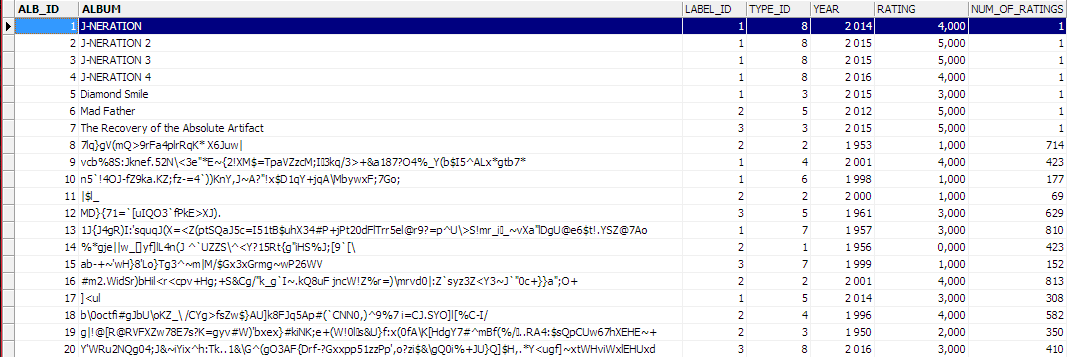
\includegraphics[width=\textwidth]{res}
	\caption{Результат генерации в таблице albums}
	\label{pic:res}
\end{figure}

\begin{figure}[H]
	\centering
	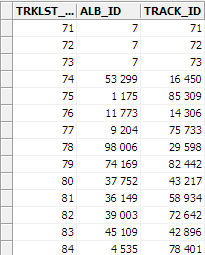
\includegraphics[width=0.3\textwidth]{restrk}
	\caption{Результат генерации в таблице tracklists}
	\label{pic:restrk}
\end{figure}